\chapter{Wave mixing in Bose–Einstein condensates}\label{chap:wave_mixing}

This chapter talks about the experiment as well as wave mixing results, both theoretical and experimental

\section{Development of a cold atom physics experiment}\label{chap:experiment}
\begin{itemize}
\item Describe how the apparatus was developed over time, what it was designed to do and everything we learned along the way. Include vacuum system design and bakeout, optical setups, atomic transport, etc. Not comprehensive, as I have not played a large role in much of the development of the appratus itself.

\item Dual species apparatus
\item -> Vacuum chamber and bakeout
\item Research visit report
\item ->
    Describe setup of Tübingen experiment (despite lack of results). It's a simple MOT setup, so describing it includes details of optics required for a MOT, which I didn't work on in the Monash apparatus, so this is a good place to describe everything that goes into a MOT experimentally. Include full optics layout I designed.
    \item -> Optics setup
    \item -> [include layout diagram of setup I designed]
\end{itemize}

\subsection{Vacuum system}
Our vacuum system comprises three chambers---two \emph{source} chambers and a central chamber. These sections are separated by differential pumping tubes, which are simply small tubes that restrict the passage of gas between the chambers\footnote{This works very effectively at very low pressures due to the fact that atoms very rarely collide with each other---and so even a factor of a thousand difference in pressure across the tube results in very little pressure-gradient force on the gas.}.

After assembly of the vacuum system, we constructed an oven around it and baked it out at approximately 200$^\circ$C for about two weeks. This increases the rate of outgassing from the interior surfaces, decreasing the extent to which later outgassing of water and hydrogen can limit our pressure. After bakeout the system's pressure was measured with a residual gas analyser (\textsc{rga})to be in the vicinity of $10^{\textrm{{-11}}}$ Torr. This was in the central chamber, which was and still is being pumped by two ion pumps and a titanium sublimation pump.

During the bakeout, the two side chambers were being pumped on by a turbomolecular pump, which was removed after baking was complete. This pumping was required to remove the products of outgassing in those chambers since the conduction to the central chamber through the differential pumping tubes is so poor.

\begin{figure}
\begin{center}
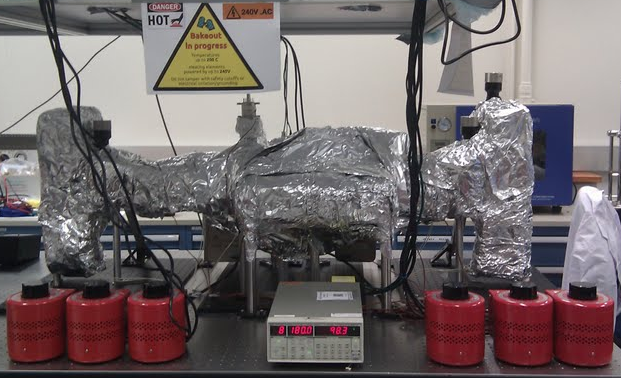
\includegraphics[width=0.8\textwidth]{figures/unsorted/bakeout.png}
\caption{\label{fig:bakeout}The temporary oven built around the vacuum system during bakeout. Temperatures were controlled with variacs providing variable voltage to the heater tape, and temperatures were monitored using thermocouples and an \textsc{SR}630 thermocouple monitor set to cut off the power if the temperature went too high. The \textsc{SR}630 was also being polled constantly over the network so that the bakeout status could be monitored remotely.}
\end{center}
\end{figure}

After bakeout, the two side chambers\footnote{Which can be sealed from the central chamber with gate valves.} were brought up to atmospheric pressure with dry nitrogen\footnote{Which comes off the interior surfaces without much baking, and if fact protects the system from other---more difficult to remove---contaminants such as water from depositing on the surfaces.}, and ampoules of the alkali metals we'll be using in our experiments---rubidium and potassium---were inserted. After pumping down and lightly baking once more, two metal weights that had been magnetically suspended above the ampoules were released and~---~after a few attempts---used to break the ampoules open. Heating elements on both chambers\footnote{Operating under a safety and control system written on embedded electronics by Phil Starkey.} have since been heating the metals to near their melting points\footnote{$39^\circ$C and $64^\circ$C for rubidium and potassium respectively.}, which should, based on the known dependence of the metals' partial pressures on temperature, provide a background pressure of approximately $10^{-6}$ Torr \cite{steck_rubidium_2010, tiecke_properties_2011}.

Unfortunately it seemed that the pressure of hydrogen in the rubidium source chamber had been increasing since the bake, as recently noticed by \textsc{rga} measurements of hydrogen in the central chamber, which diminished upon closing the gate valve in between. To address this, we are modified that end of the vacuum system to include an ion pump. This was possible to do without having to break existing vacuum. Only the rubidium end was affected, presumably because it has a o-ring valve (where the pump during bakeout was attached) which a) could not be baked as hot as the rest of the system and b) may have been leaking. The addition of the new pump and a short bake of the local area appears to have alleviated the problem (Figure \ref{fig:lifetime}).

\begin{figure}
\begin{center}
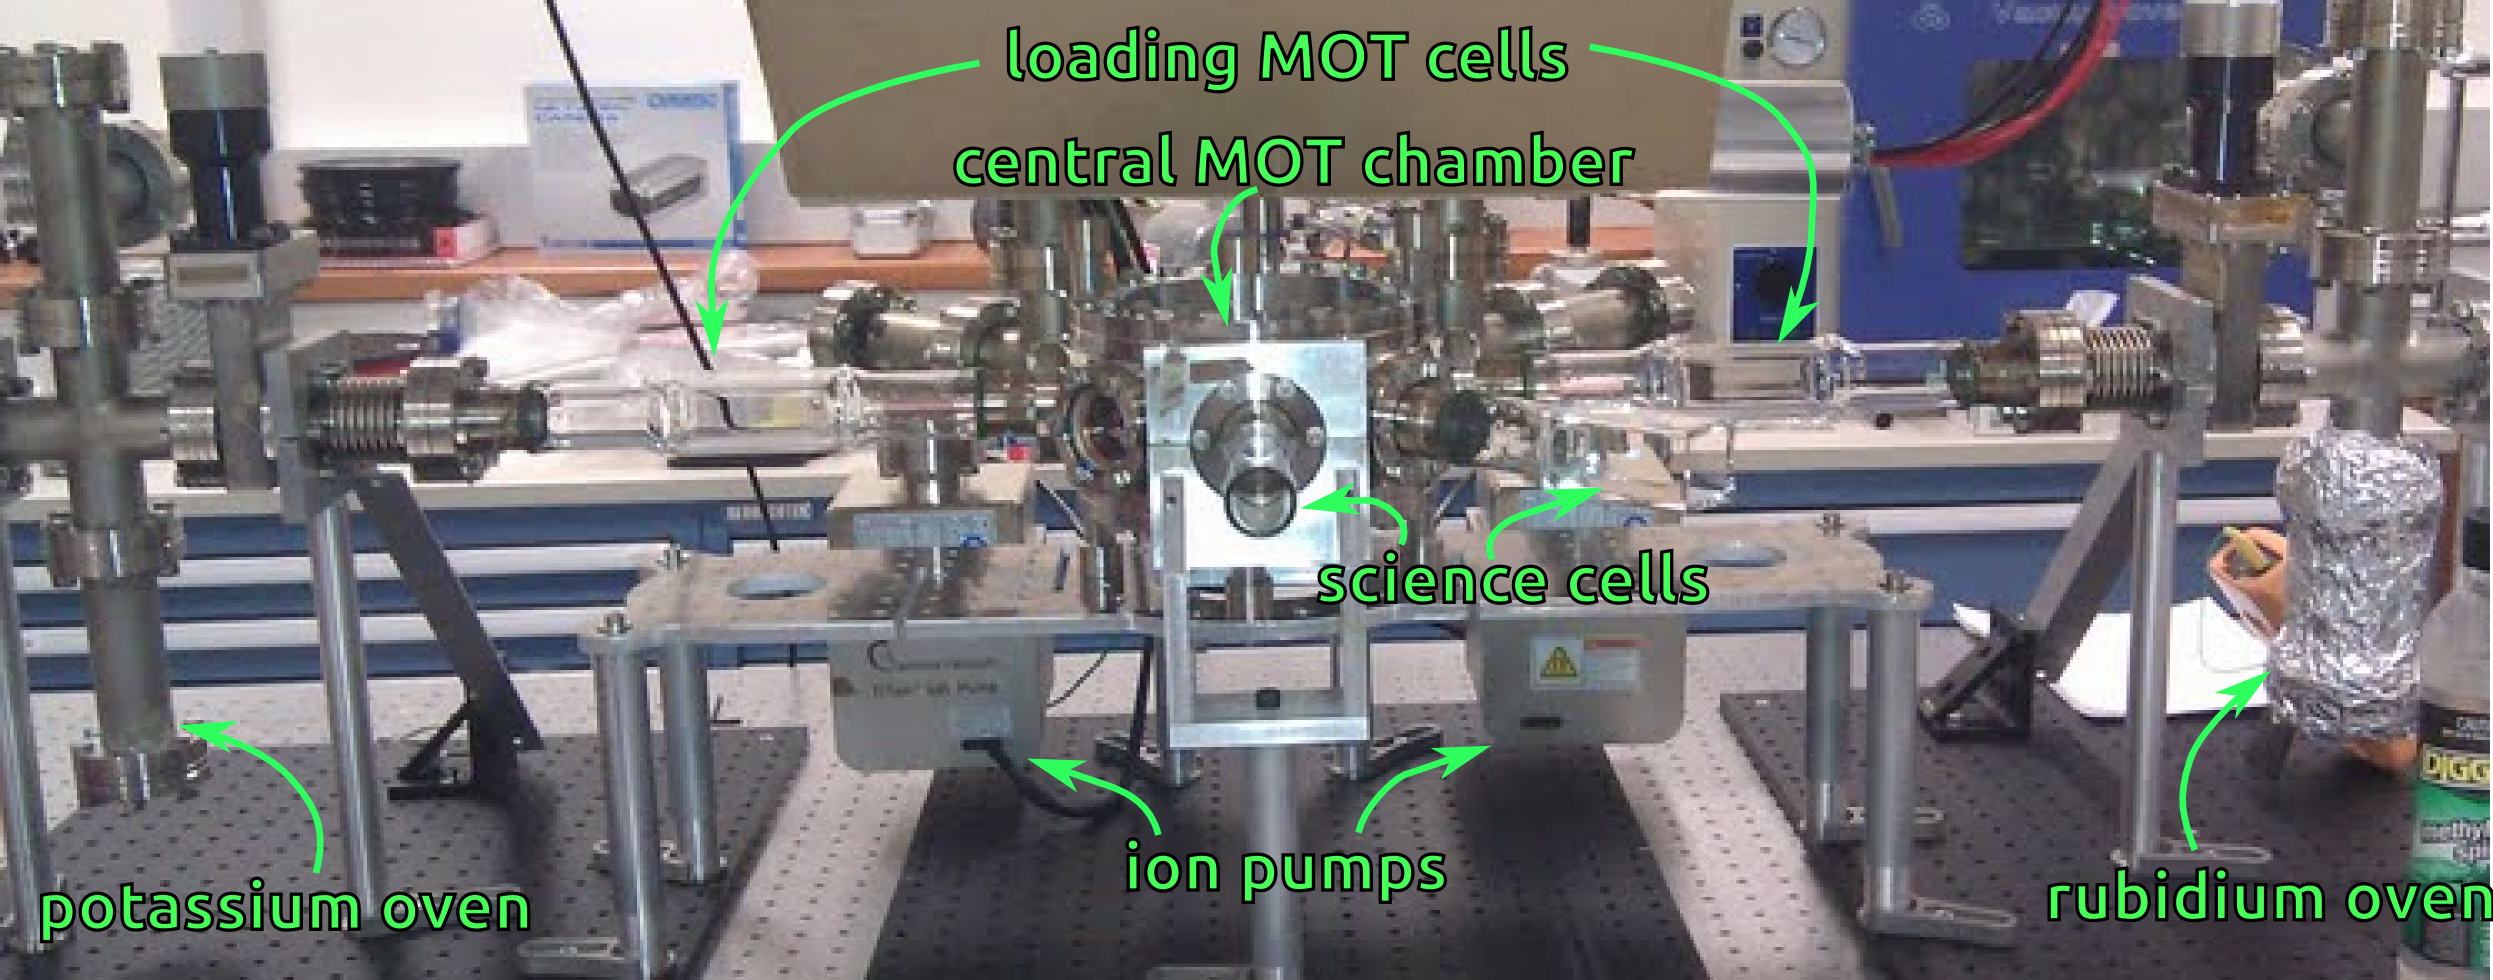
\includegraphics[width=0.9\textwidth]{figures/unsorted/vacsystem.png}
\caption{\label{fig:vacsystem}The vacuum system after bakeout and insertion of alkali metal ampoules.}
\end{center}
\end{figure}

\begin{figure}
\begin{center}
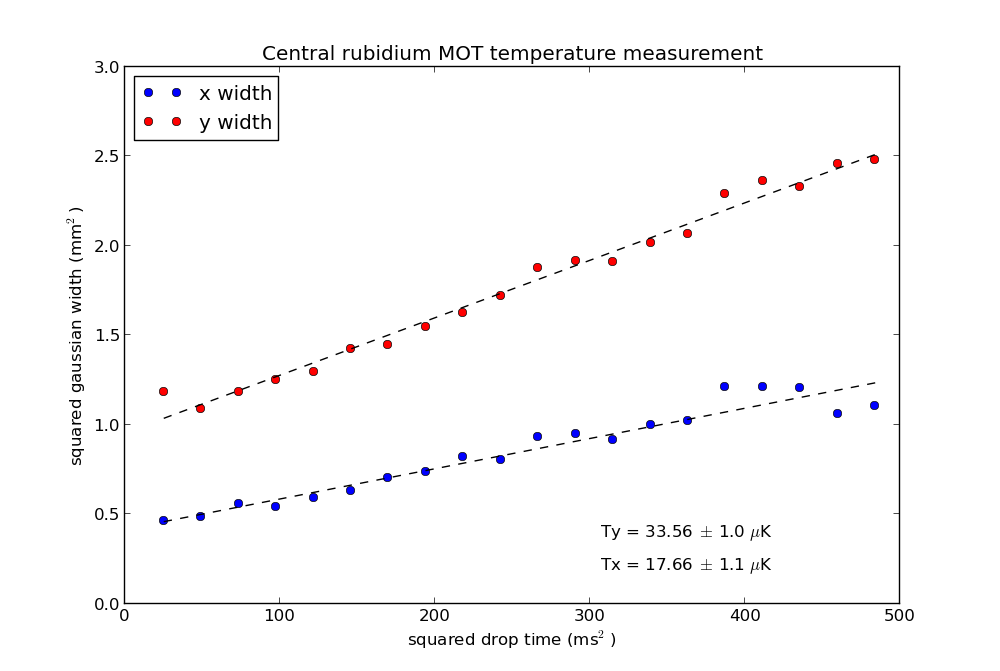
\includegraphics[width=0.8\textwidth]{figures/unsorted/temp.png}
\caption{\label{fig:temp} A temperature measurement of the rubidium \mot\ in the central chamber. Temperature was determined by measuring the rate of expansion of the atom cloud when released from the magnetic trap. The magnetic trap was switched off, and then the atoms were imaged with a pulse of light after being allowed to expand for a time. The expansion time was varied and compared to the size of the condensate in order to determine the expansion rate, which has a simple relation to temperature. This temperature was obtained without a polarisation gradient cooling stage, however it is lower than the Doppler limit ($\approx 140 \,\upmu$K) due to some \textsc{pgc} taking place regardless.}
\end{center}
\end{figure}

\begin{figure}
\begin{center}
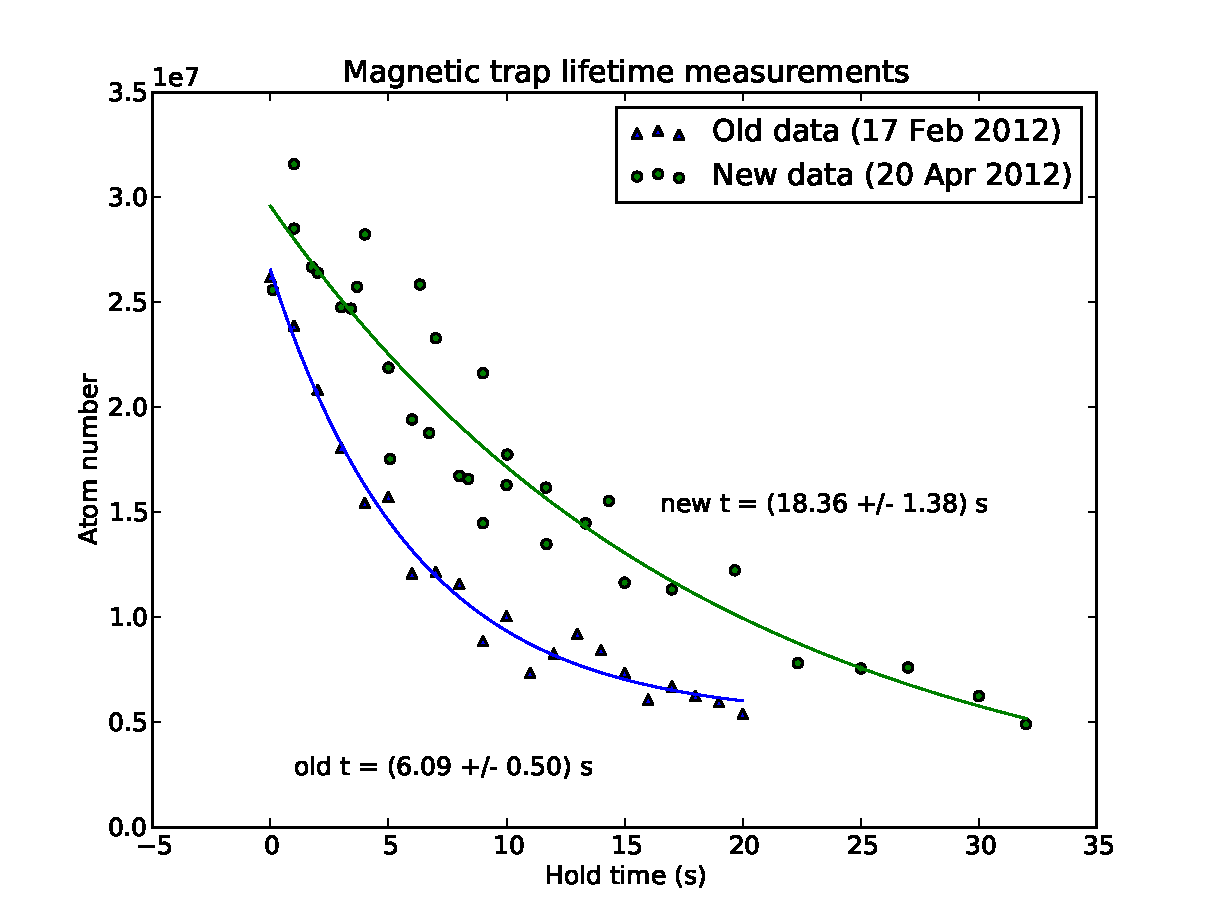
\includegraphics[width=0.8\textwidth]{figures/unsorted/lifetimes.pdf}
\caption{\label{fig:lifetime} A measurement of the magnetic trap lifetime before and after an extra pump was added to the rubidium source chamber. The trap lifetime was measured by turning off the cooling beams such that atoms were trapped only magnetically, then waiting a time before fluorescence imaging with a pulse of light. By computing the number of atoms remaining from the fluorescence, and comparing with the delay time, the decay rate due to collisions with background gases was determined. An increase in the atom number has since been obtained, resulting in $1.2\times10^8$ atoms, with the same trap lifetime.}
\end{center}
\end{figure}

\subsection{Cooling and trapping of atoms}

\mot s have been formed in both source chambers using anti-Helmholtz magnetic coils and Doppler beams. The cooling beams are circularly polarised in order to pump the cooling transition of the atoms, and there is also repump light to move atoms back into the cooling cycle when they decay to an undesired groundstate. Both \mot s collect atoms from the relatively high pressure background gas from the alkali ovens in the source chambers, before those atoms are transported to the central chamber.

\subsection{Transport of atoms}

The initial idea was to use magnetic transport to move atoms into the central chamber of the vacuum system. Due to a delay in the construction of magnetic coil control electronics, another alternative was investigated in the meantime---the push-beam method. Magnetic transport, once attempted, proved to be less efficient (due high collisional losses during the slow transit), as well as technically challenging, and so we have continued to use the push-beam method, in which atoms are given momentum by resonant light from a single beam. Atoms are pushed by this beam into the central chamber, where they are caught in the \mot\ there. This has been done for rubidium but not yet for potassium.


\section{Off-resonant four wave mixing}

    [copy from poster basically]

    \subsection{Experimental methods}

    \null\newpage
    \null\newpage
    \null\newpage
    \null\newpage

    bragg pulses etc
    \subsection{Results and analysis}

    \null\newpage
    \null\newpage
    \null\newpage
    \null\newpage

Describe the wave mixing experiments and their results, compare with the simulations I performed and provide the simplified three-level model explaining the results.

\section{Spin wave mixing}
Show results of spin wave mixing simulations, including scaling behaviour with increasing c2.

\null\newpage
\null\newpage
\null\newpage
\null\newpage